\documentclass[a4paper]{article}
\usepackage{amsmath}
\usepackage{amsfonts}
\usepackage{mathabx}
\usepackage{amsthm}
\usepackage{amssymb}
\usepackage{framed}
\usepackage{relsize}
\usepackage{subfig}
\usepackage{graphicx}
\usepackage{wrapfig}
\usepackage{titling}
\usepackage[margin=1.5in, top=1in, bottom=1in]{geometry}
\graphicspath{{images/}}
\usepackage{subcaption}
\usepackage{enumerate}
\usepackage{booktabs}
\setlength{\droptitle}{-8em}
\usepackage[usenames,dvipsnames]{color}
\usepackage{tikz}
\usepackage{listings}
\usepackage{fancyhdr}
\usepackage{minted}
\usepackage{tcolorbox}
\usemintedstyle{emacs}
\setlength{\parindent}{0pt}
\pagestyle{fancy}
\fancyhf{}
\fancyhead[R]{Michael Redman, CID:\ 00826863}
\fancyfoot[C]{\thepage}
\begin{document}
\title{Machine learning --- Coursework 2}
\author{Michael Redman, CID:\ 0082686\textbf{3}}
\date{March 2017}

\maketitle

\section*{Question 1}

Gaussian mixture models and the K-means algorithm are both examples of clustering. Given an array of pixels each represented by a point in 3-dimensional colour space we can obtain a segregation of the image by assigning each pixel to one of k clusters --- reducing the dimensionality of the data by representing each pixel by a label instead of a colour in $\mathbb{R}^3$. 

In both methods this is done by assigning the points to clusters which are represented by a centroid (and in the Gaussian case a covariance matrix) based on which of these centroid is---in some sense---closest to the point to be classified. In the case of K-means this is typically defined as the euclidean distance to the centroid and in Gaussian mixture models by the cluster which, weighted by the estimated mixture proportion of the cluster, maximises the likelihood of the point.

The K-means algorithm simply consists of iteratively assigning each point to the closest cluster mean and then calculating the new mean of each cluster. However, ommited from this procedure, is what is our starting assignment of the points to the clusters? This is a matter of some study, but in this project we simply randomly assign the points to each cluster at the start. The class \emph{KMeans} implements this K-means procedure for a given set of points and number of clusters.    

In Gaussian mixture models we need a way of fitting our model to the data. Here we used the EM-algorithm, which consists of calculating the values of the parameters which maximise the conditional expectation of the log-likelihood where we condition on the previous values of our parameters. For a simple Gaussian mixture model this log-likelihood is linear in our parameters so we are able to find the optima seperately for each parameter. So, after assigning initial labels to each point, we begin by finding the conditional memebership probabilities of each point\footnote{Much of the notation used here is borrowed from the Wikipedia page on the EM-algorithm, generalized to the k-mixture case.},
\begin{equation}
T_{j,i}^{(t)} = P(Z_i = j | X_i = x_i, \theta^{(t)}) = \frac{\tau_j^(t) f(x_i | \mu_j^{(t)}, \Sigma_j^{(t)})}{\sum_{l=1}^k \tau_l^(t) f(x_i | \mu_l^{(t)}, \Sigma_l^{(t)})}
\end{equation}

where $Z_i$ is label which represent which cluster the $i$th point belongs to and $\tau_j$ is the proportion of points which belong to the $j$th cluster. Note that this is the probability which we will take expectations with respect to. Skipping over the calculation of this expectation, we obtain the following optima -- which will serve as the new estimated of the parameters:

\begin{gather}
\tau_j^{(t+1)} = \frac{1}{n} \sum_{i=1}^n T_{j, i}^{(t)} \\
mu_j^{(t+1)} = \frac{\sum_{i=1}^n T_{j,i}^{(t)} x_i}{\sum_{i=1}^n T_{j,i}^{(t)}} \\
\Sigma_j^{(t+1)} = \frac{\sum_{i=1}^n T_{j,i}^{(t)} (x_i - \mu_j^{(t+1)}){(x_i - \mu_j^{(t+1)})}^T}{\sum_{i=1}^n T_{j,i}^{(t)}}.
\end{gather}

We see that our parameters can be calculated with relatively simple operations using the calculated values of $T$. Like before the inital values of the parameters could be a point of discussion, but in my implmentation I simply set the initial values of $\tau$ to all be equal, the values of $\mu$ to be $k$ randomly selected points in the dataset (sampled without replacement) and the inital covariance matricies to be diagonal with a large variance to prevent undesirable local optima.

The Gaussian mixture model is implemented in the class GaussianMixture, which is well documented. The calculations of the matrix $T$, which we call expectation in the class, and the inner product used in the updating of $Sigma$ are both very computationally intensive so were rewritten in Fortran to obtain workable performance. This code, included in the appendix, will need to be compiled with {\bf f2py} (including LAPACK flags) in order to be importable by Python --- an example makefile is included alongside the code.

Both the KMeans and Gaussian mixture model algorithms are iterative and need criteria for when to stop, for this project I manually inspected the values of the parameters between iterations until it was clear that the values had stabalized. 

So we begin with the image data, flatten the array and apply the two methods for varying values of $k$. The resulting segregations of the image are reshape and diplayed in figure x. We see that both of the methods produce a desirable classification for most values of $k$. The Gaussian mixture model produces clean demarcations around the cells which are ``well filled'', while the K-means algorithm produces less clean lines but is free from the noise of the Gaussian mixture where points clearly not a part of a cell have been spurriosly assigned to the same class as the cells --- presumably because one of the Gaussian mixtures has settled on a covariance matrix with larger variance values compared to the other mixtures (something which is not possible in K-means). 

As we are going to use a Gaussian mixture model again for the counting of clusters we will use the K-means segregation with $k = 3$ as the leptokurtic nature of the GMM segregation will handicap the fitting of a mixture of Normal distributions by overestimating the covariances.

We start by calculating which cluster has the fewest members, this will be the cluster containing the points that are determined to be within the disc-shaped section of the cells, and find the coordiantes of each of the points in this cluster --- these will be our covariates. We now split our points randomly into train and test portions. Fitting a Gaussian mixture model for a range of $k$ values to the train set we calculate the log-likelihood of the test set under the fitted model. This is first done at a coarse level, in increments of 10, and then at the individual level around the optima of the log-likelihood. The results of the individual level optimization can be seen in fig y.

We see that we have optimal $k$ value of X, this is what we take as our estimate the number of cells in the image. Taking the values of the $\mu_j$ for the $k = X$ case and overlaying over the points obtained via segregation we obtain fig z. It's clear from this image that the EM-alogrithm has not been able to find the cluster in a few cases, and in others the irregular shapes of the discs has meant multiple normals fit better than a single normal with larger covariance. 

Overall, these two effects have counterbalanced each other and the whole procedure has worked quite well. The segregation procedure certainly worked excellently for both methods and the counting stage worked as well as can be expected. The EM-algorithm's tendency to become stuck in local optima should be expected for so many mixture components. Perhaps a less naive method would be to place explicit priors on the hyperparameters, such as a hierachical prior on the covariance matricies to provide shrinkage or a non-local prior to penalize small distances between means of the mixtures. Also a method of fitting the models which is less likely fall victim to the complex geometry of Gaussian mixture models, such as Hamiltonian Monte Carlo, would probably obtain more accurate results.

\begin{figure}[p]
\centering
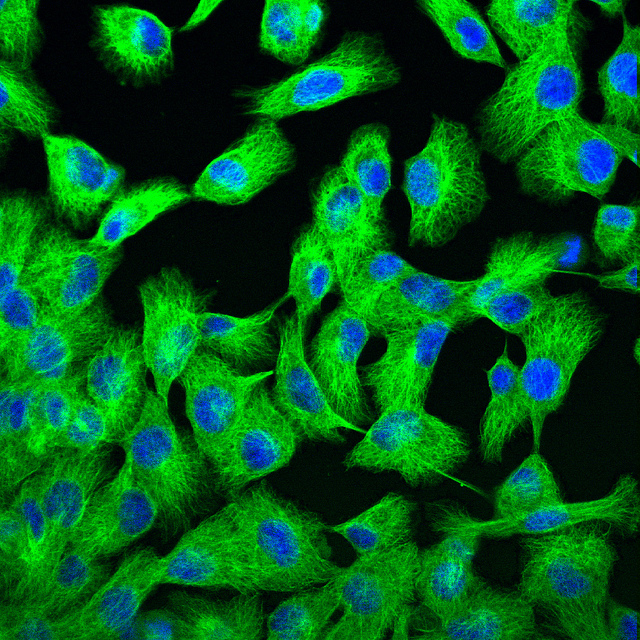
\includegraphics[width=0.4\textwidth]{original}
\captionof{figure}{Original image}
\label{fig:original}
\end{figure}

\begin{figure}[p]
\begin{minipage}{0.32\textwidth}
\centering
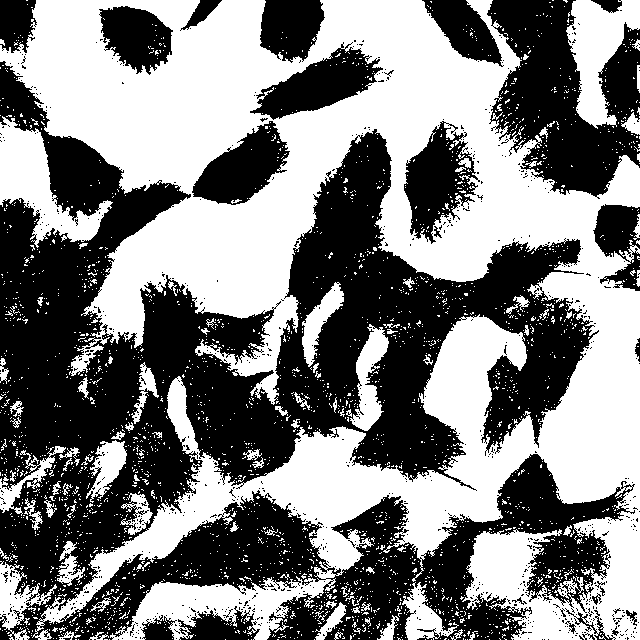
\includegraphics[width=1\textwidth]{km2}
\captionof*{figure}{k = 2}
\label{fig:km2}
\end{minipage}%
\begin{minipage}{0.32\textwidth}
\centering

\includegraphics[width=1\textwidth]{km3}
\captionof*{figure}{k = 3}
\label{fig:km3}
\end{minipage}%
\begin{minipage}{0.32\textwidth}
\centering
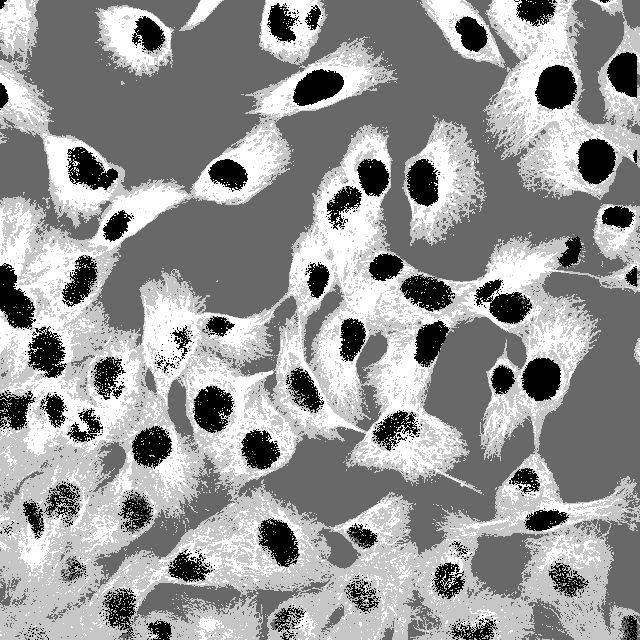
\includegraphics[width=1\textwidth]{km4}
\captionof*{figure}{k = 4}
\label{fig:km4}
\end{minipage}%
\captionof{figure}{K-Means clustering}
\end{figure}

\begin{figure}[p]
\begin{minipage}[b]{0.32\textwidth}
\centering
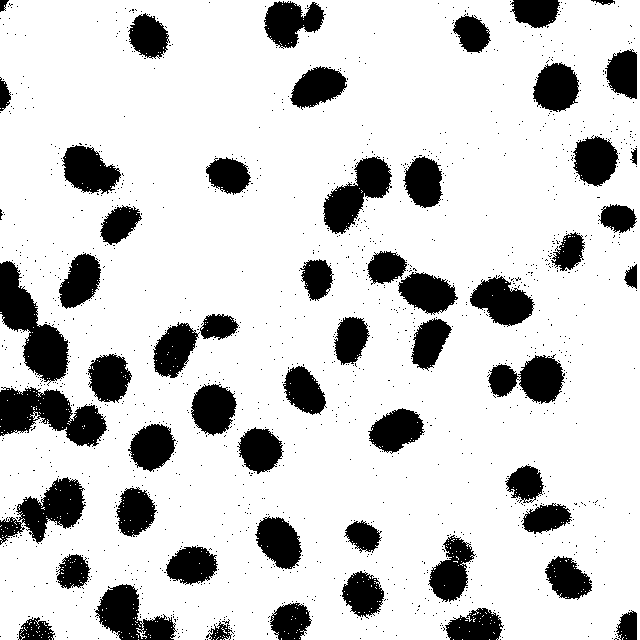
\includegraphics[width=1\textwidth]{gmm2}
\captionof*{figure}{k = 2}
\label{fig:gm2}
\end{minipage}%
\begin{minipage}[b]{0.32\textwidth}
\centering
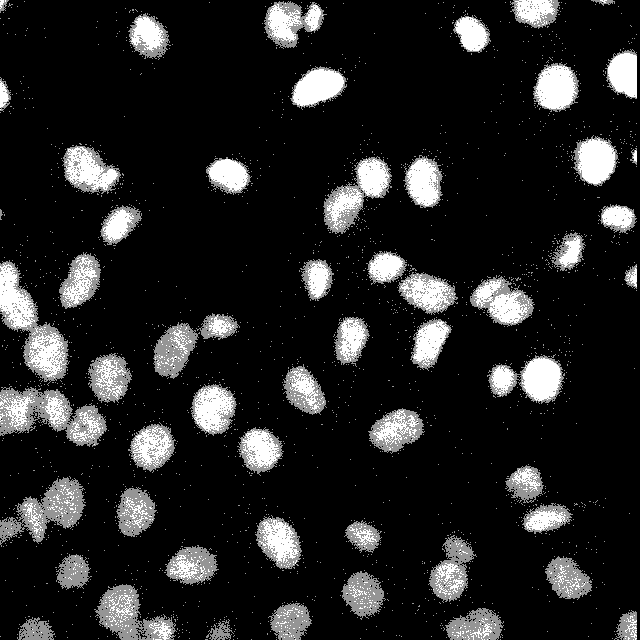
\includegraphics[width=1\textwidth]{gmm3}
\captionof*{figure}{k = 3}
\label{fig:gm3}
\end{minipage}%
\begin{minipage}[b]{0.32\textwidth}
\centering
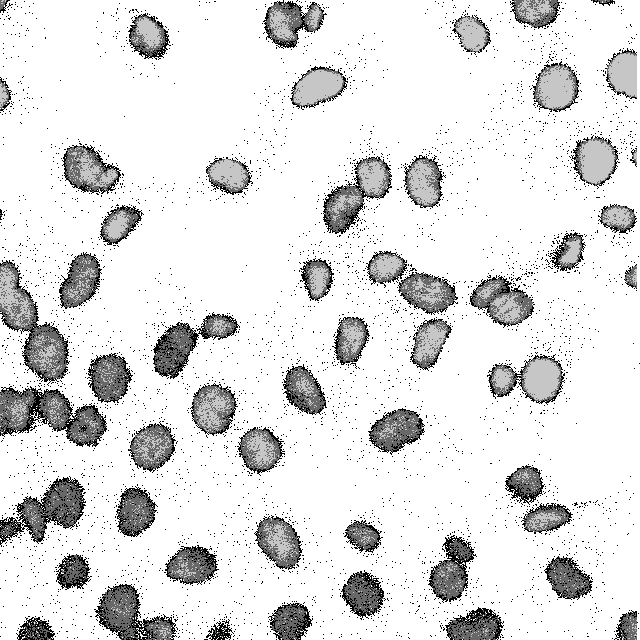
\includegraphics[width=1\textwidth]{gmm4}
\captionof*{figure}{k = 4}
\label{fig:gm4}
\end{minipage}%
\captionof{figure}{Gaussian mixture model clustering}
\end{figure}

\begin{figure}[p]
\begin{minipage}[b]{0.5\textwidth}
\centering
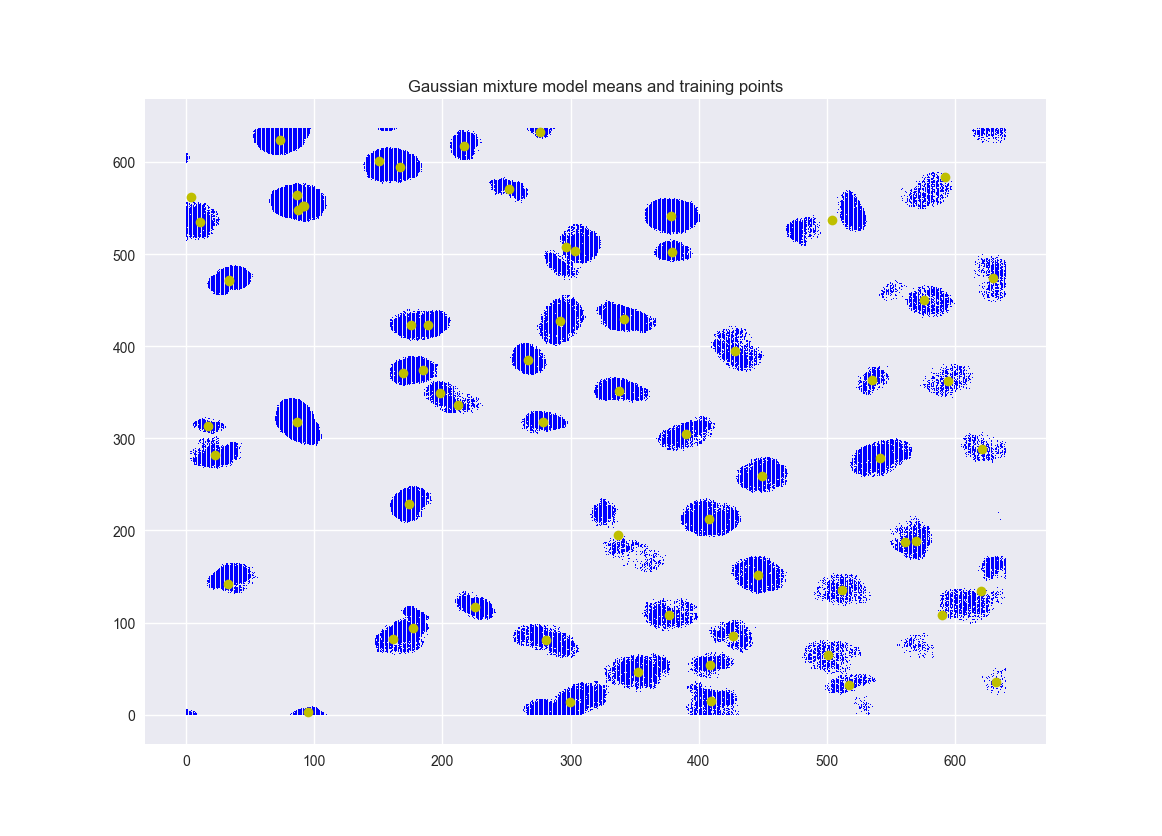
\includegraphics[width=0.95\textwidth]{mixmu}
\captionof{figure}{Mean locations}
\label{fig:mixmu}
\end{minipage}%
\begin{minipage}[b]{0.5\textwidth}
\centering
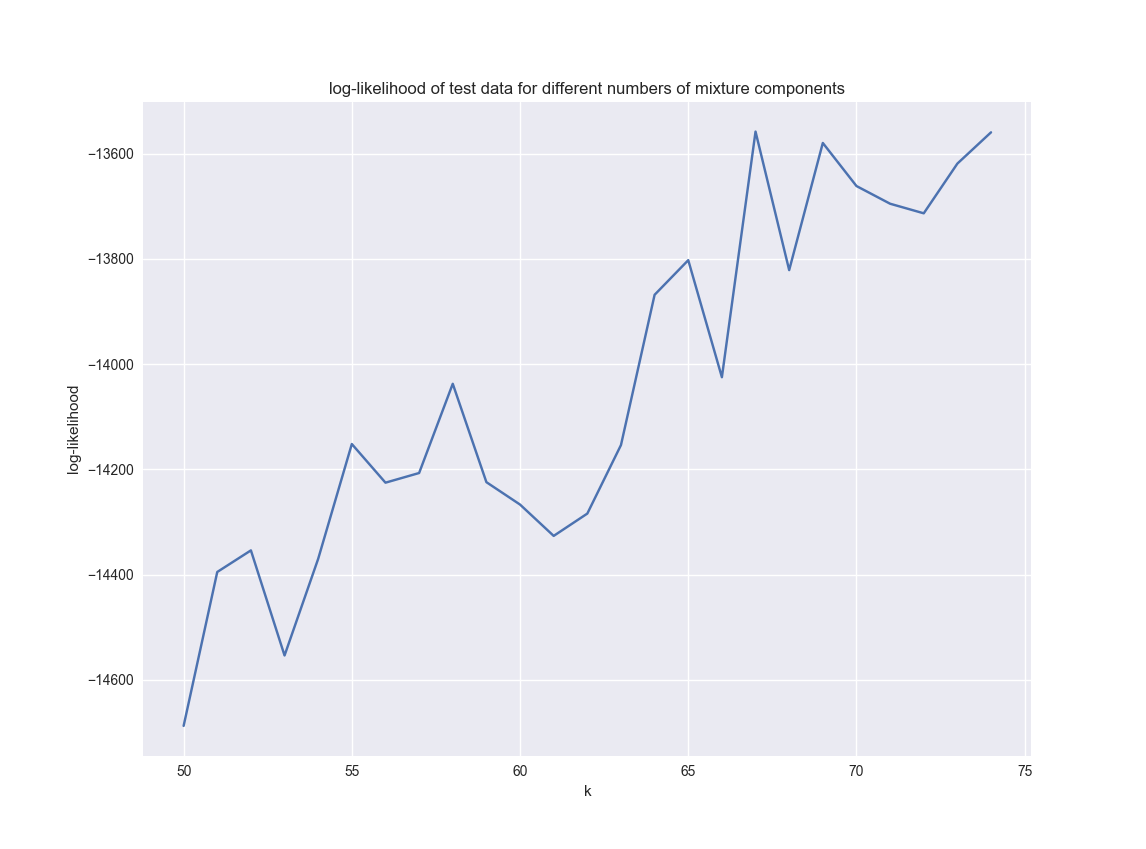
\includegraphics[width=0.95\textwidth]{kvals}
\captionof{figure}{Log-likelihood calculations}
\label{fig:kvals}
\end{minipage}%
\captionof{figure}{Counting procedure mixture model calculations}
\end{figure}

\newpage

\section*{Question 2}

Say we wish to fit the model
\begin{equation}
y_i = f({\bf x}_i) + \epsilon_i
\end{equation}

where our dependent variable is modeled as coming from an underlying function of the covariates with noise. If our function can be decomposed into a finite linear sum of our covariates, transformed by some kernal function(s), then we are doing linear regression:
\begin{equation}
f(x) = \sum_{m=1}^M \theta_m \phi_m(x) = \theta^T \phi(x).
\end{equation}

The frequentist way of estimating the $\theta_m$ would be to find the values that maximise the likelihood of the data. However, viewing this model from a generative perspective, this modal estimate often gives non-typical values. Using a Bayesian approach we can place a prior over the values of $\theta$, which allows us to incorporate any additional information we believe about the structure of the model. Not only does this provide shrinkage, but the explicit computation of a posterior distribution enables us to work with expectations of model statistics. This gives both more robust estimatimation of the $\theta_m$ and allows us to calculate their marginal variances. 

Say we place an independent Gaussian prior over each of the weights
\begin{equation}
p({\bf\theta}) \sim N(0, \alpha I_M)
\end{equation}

then we can calculate the posterior as follows
\begin{equation}
p(\theta|X, y, \alpha) \propto p(y | \theta, X, \alpha) \cdot p(\theta).
\end{equation}      

This formulation can also be viewed from the perspective of a Gaussian process. The prior placed on the $\theta_m$ can allows us a direct interpretation of the covariance between two points
\begin{align}
K(x, x^*) &= E[f(x), f(x^*)] \\
          &= \phi{(x)}^T \Sigma_\theta \phi(x^*) \\
          &= \alpha \phi{(x)}^T I_M \phi(x^*)
\end{align}

In fact Gaussian process can be viewed a limiting case of Bayesian linear regression as every kernal function can be decomposed into an infinite sum over the eigendecomposistion of the basis functions
\begin{equation}
K(x, x^*) = \sum_{i=1}^\infty \lambda_i \varphi_i(x) \varphi_i(x^*)
\end{equation}

we recognize that this summation form could be found for Gaussian noise linear regression by diagonalizing the covariance matrix. 

Now we turn to the climate data. Plotting the data we see two things: 
\begin{enumerate}
\item At the macro level the CO2 data is positively correlated with the previous values,
\item There is a yearly seasonal oscillating trend.
\end{enumerate}

We use these two facts to construct an appropriate kernal function to represent the correlation between time points. The general trend is best captured using a squared exponential kernal function which allows for exponentialy decaying autocorrelation and the seasonal trend is captured using a sinusoidal kernal function which allows a periodicity in the autocorrelation. We combine these two to make our mixed kernal function
\begin{equation}
K(x, x^*) = \alpha_1 \exp{\left(-0.5 \cdot \frac{{(x - x^*)}^2}{\lambda^2} \right)} + \alpha_2 \exp{\left(-2 \cdot \sin^2\left(\frac{x - x^*}{3.81}\left)\right)}
\end{equation}

where we have chosen the figure $3.81$ to make the periodicity annual ($12/\pi$). 

Now we need to estimate the remaining parameters of the model. The way we do this is by maximising the log-likelihood function of the equivalent multivariate Gaussian on our data. However if we naively estimate the Gaussian noise standard deviation along with the other parameters of our kernal function then we will run into issues. Due to the nature of this kernal function if the standard deviation is estimated via MLE then it will blow up and we will be explaining the variation of the data as though it were simply noise and we will not fit the other parameters accurately. So in order to estimate the variance I took partitions of the data, where each partion contains the same number of consecutive points, and calculated the variance of each partition and then averaged them. This is an attempt at ``zooming in'' to the data until we're only looking at noise. This eas done for multiple partition sizes to get an idea of the plausable values of the standard deviation. 

The remaining parameters were estimated by maximizing the log-likelihood via BFGS. The log-likelihood for a Gaussian process is as follows,
\begin{equation}
\mathcal{L} = \log p(y|\theta) = - \frac{1}{2} \log \det C(\theta) - \frac{1}{2} y^T {[C(\theta)]}^{-1} y - \frac{N}{2} \log{(2\pi)}
\end{equation}
where
\begin{equation}
C(\theta) = K + \sigma^2 T. 
\end{equation}

The functions for the calcuation of covariance matrcies for this kernal is written in Fortran for speed and used for the maximization procedure.

We also wrote a function called \emph{kernal} which calculates the mean and covariance matrix for a set of points, given another set of points where we have the response values. We use the following derived quantities
\begin{gather}
\mu_T = K_{TN} {(K_N + \sigma^2I)}^{-1} y \\
\Sigma_T = K_T - K_{TN} {(K_N + \sigma^2I)}^{-1} K_{NT}
\end{gather}

We fit the model to the data and predict the values of a set of points into the future from the observed data. We see, evaluating for multiple $\sigma^2$ values we previously deemed plausable, that there is a critical point around $\sigma^2 = 0.75$ where the projection undergoes a qualititive change in behaviour. Before this point the projection is fit very tightly to the trend of the observed data and has very limited variance around its projected values. However at and after $\sigma^2 = 0.75$ the model believes that the underlying function has a much greater degree of freedom, and there is less autocorrelation allowing the projection to eventually regress toward the mean. Fig x shows the values $\pm 1$ standard deviation from the projected points. Why this point is so critical probably has to do with the almost multi-modality of the likelihood function of the parameters --- within the typical set the likelihood is reasonably flat so small changes in the $\sigma^2$ variable which changes the ``likelihood surface'' only slightly can still lead to huge changes in the values of the parameters which optimize the likelihood. 

\begin{figure}[p]
\begin{minipage}[b]{0.5\textwidth}
\centering
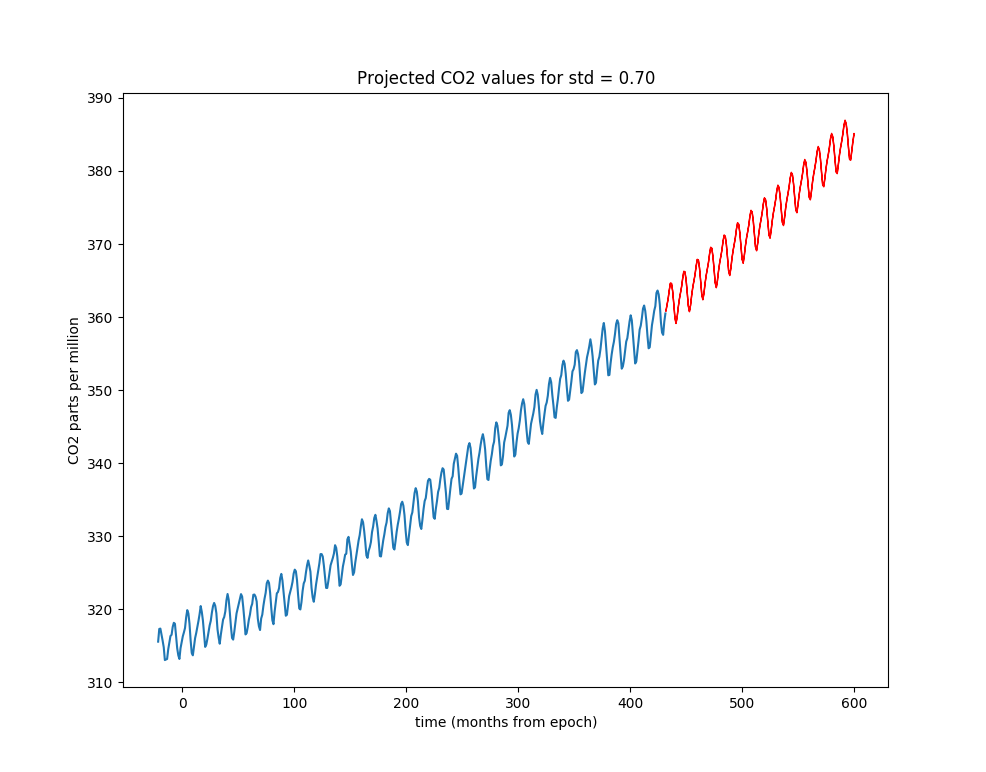
\includegraphics[width=\textwidth]{std70}
\label{fig:std70}
\captionof*{figure}{$\sigma^2 = 0.70$}
\end{minipage}%
\begin{minipage}[b]{0.5\textwidth}
\centering
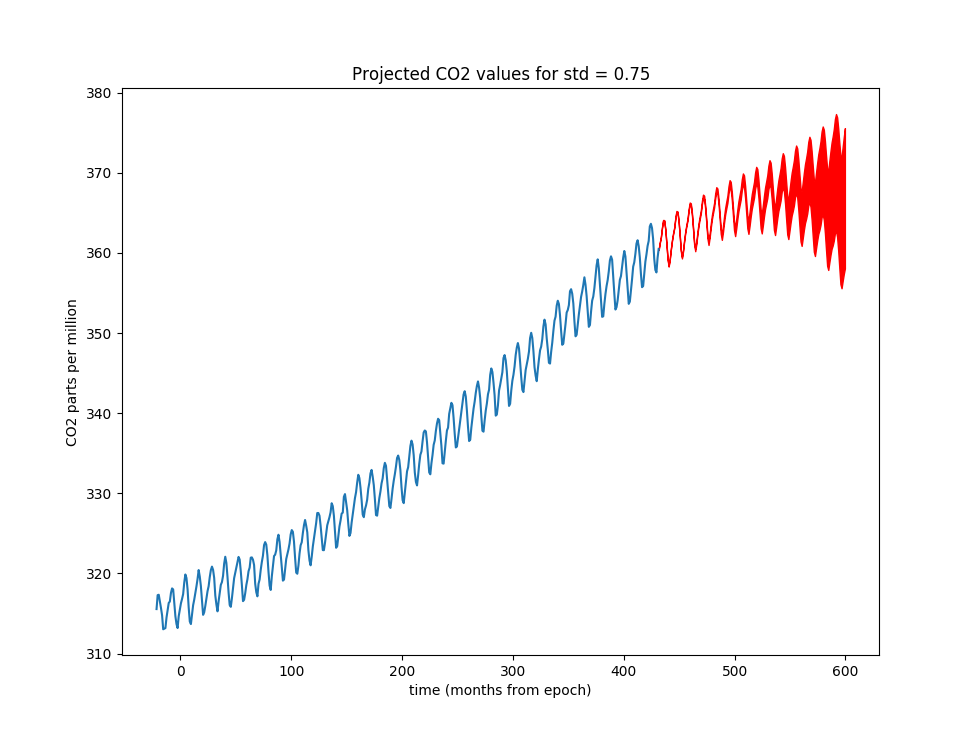
\includegraphics[width=\textwidth]{std75}
\label{fig:std75}
\captionof*{figure}{$\sigma^2 = 0.75$}
\end{minipage}
\captionof{figure}{Projected values of climate data for different $\sigma^2$ values}
\end{figure}      

\section*{Question 4}

To predict the Bitcoin prices we again used a Gaussian process, but this time without the seasonality component. Like before we took partitions of the data and used it to find an estimate of the variance for the Gaussian noise underlying the process. After finding a reasonable value of $\sigma^2 = 0.1$ we tried to use a maximum likelihood approach for the estimation of the length scale and $\alpha$ coefficient but they led to issues where the high variance at a low level caused the values to have much to large spreads. We might expect to have such issues as financial time series are often most appropriately modelled as Brownian motion which, due to its self-similarity, has infinite variance. So perhaps if the underlying function that is not well behaved in some sense then we won't obtain reasonable parameter estimates via MLE.

Instead we devise a trading strategy first and optimize the parameters with respect to this strategy. The one we use is very simple, 
\begin{enumerate}
\item We select a holding period that represents the length of projection that we wish to optimize for.
\item Given a projected price at the end time point, if the projected price is above the price at which we can buy at (at the next available time that we can buy) then we buy at that price and sell at the end of the holding period.
\item Likewise if the projected price is below that of the price we can sell at (at the next available time that we can sell) then we sell at that price and buy the bitcoin back at the end of the holding period. 
\item We weight how much Bitcoin we buy or sell relative to the relative difference between the projected price and the buy/sell price. So if we project a large movement then we will buy/sell commensurately more.
\end{enumerate}

This isn't a very realistic strategy for many reason, including
\begin{enumerate}
\item Just because there is a bid/ask doesn't mean we can sell/buy in the amounts that we want to. Orders have volume as well as direction!
\item We might want to trade multiple overlaping trades over the length of the holding period --- there is no guarentee we will remain liquid enough over that time to execute the trades we want to.
\item If we have a concrete projected price then more complex financial instruments (options exist for Bitcoin apparently) can be used to make greater profit from the additional clarity we have over simply up down, (e.g. long/short butterfly).  
\end{enumerate}

However it provides a basis with which to work with. To estimate the parameters we manually tried a range of values while evaulating our trading strategy for the first half of the time series, due to the nature of what we are fitting there will be significant issue with overfitting so I chose to use heavily rounded values (settling on $\alpha = 0.1, \lambda = 1000$). The projected values using these values for a wait time of 50 time units, and trading every 200 time units, are shown in fig z --- we see that they are wildly inaccurate but what matters is if it is accurate enough to make money using our trading strategy. Evaluating the trades using these projections we see 

\newpage

\section*{Appendix}

The project as a whole can be found at https://github.com/michaelaredman/ML-Coursework --- It may be easier to use the Python files on the Github repo if you want to run anything as some of the import statements are dependent on the file names containing the code being correct. \\
 
Note: Some of the minor calculations and plotting in this project were made in a REPL environment and so are not included in this appendix.

\subsection*{Imperative code}

\subsubsection*{Question 1}

I don't recommend running this whole block as it may take a while. The code is mostly self-explanatory, run the bits of interest seperately.

\begin{minted}[breaklines]{python}
import numpy as np
import time
import random
from matplotlib import pyplot as plt
from scipy.optimize import minimize
import pandas as pd
import seaborn as sns
from cluster import cluster as cl
from clus import *
from scipy import misc

#plt.ion()

cells_image = misc.imread('../FluorescentCells.jpg', mode='RGB')
cells = cells_image.reshape(640*640, 3)

km2 = KMeans(cells, 2)
km3 = KMeans(cells, 3)
km4 = KMeans(cells, 4)

gaus2 = GaussianMixture(cells, 2)
gaus3 = GaussianMixture(cells, 3)
gaus4 = GaussianMixture(cells, 4)

km3.iterate(15)
km3low = km3.clusters.reshape(640 ,640)
coors = np.where(km3low==0)

#km2.iterate(15)
#km2low = km2.clusters.reshape(640, 640)

#km4.iterate(15)
#km4low = km4.clusters.reshape(640, 640)

gaus2.iterate(30)
gaus3.iterate(30)
gaus4.iterate(30)
classifiedG2 = gaus2.classify(cells)
num0 = (classifiedG2 == 0).sum()
num1 = (classifiedG2 == 1).sum()
ind = 1*(num1 <= num0)
coors = np.where(classifiedG2.reshape(640, 640) == ind)

classifiedG3 = gaus3.classify()
classifiedG4 = gaus4.classify()

plt.imsave('gmm2.png', classifiedG2.reshape(640, 640))
plt.imsave('gmm3.png', classifiedG3.reshape(640, 640))
plt.imsave('gmm4.png', classifiedG4.reshape(640, 640))

plt.imsave('km2.png', km2low)
plt.imsave('km3.png', km3low)
plt.imsave('km4.png', km4low)

locs = np.vstack([coors[0], coors[1]]).T

np.random.shuffle(locs)

train = locs[:-1000, :]
test = locs[-1000:, :]
ll = []
mus = []
for i in np.arange(50, 75, 1):
    print(i)
    gmm = GaussianMixture(train, i)
    gmm.iterate(35)
    mus.append(gmm.mu)
    print("Iteration completed")
    new_ll = gmm.loglikelihood(test)
    print(new_ll)
    ll.append(new_ll)

ks = np.arange(50, 75, 1)

plt.plot(locs[:, 0], locs[:, 1], 'b,')
plt.plot(gmm.mu[:, 0], gmm.mu[:, 1], 'yo')
\end{minted}

\subsubsection*{Question 2}

\begin{minted}[breaklines]{python}
import numpy as np
import sklearn
import time
from matplotlib import pyplot as plt
from scipy import misc
from scipy.optimize import minimize
import pandas as pd
from cluster import cluster as cl

cells_image = misc.imread('../FluorescentCells.jpg')
cells = cells_image.reshape(640*640, 3)

co2_data = pd.read_csv('CO2_Mauna_Loa_Data.csv')
co2_unnorm = np.array(co2_data['co2 ppmv'])
co2 = co2_unnorm - co2_unnorm.mean()
months = np.array(co2_data['months since 1960-01-01'])

def neg_log_likelihood(y, period, lmbda, var_se, var_sin, std):
    C_theta = cl.k_matrix(months, months, period, lmbda, var_se, var_sin) + std*std*np.identity(len(months))
    evals = np.linalg.eigvals(C_theta)
    logdetC = np.real(np.log(evals).sum())
    term1 = 0.5*logdetC
    #print(term1)
    term21 = np.matmul(np.linalg.inv(C_theta), y)
    term2 = 0.5*np.matmul(y, term21)
    #print(term2)
    term3 = 0.5*len(y)*np.log(2*np.pi)
    return term1 + term2 + term3

extra = np.arange(431.5, 600)

thing = cl.kernal(months, co2, extra, 2.7e-01, 1.09, 3.05e03, 3.0e03, 2.0e3)
thing2 = cl.kernal(months, co2, extra, 2.7e-01, 1.09, 3.05e03, 3.0e03, 2.0e3)

def plotter(period, lmbda, var_se, var_sin, std):
    ker = cl.kernal(months, co2, extra, std, period, lmbda, var_se, var_sin)
    plt.plot(extra, ker[0])
    plt.plot(months, co2)
    file = 'pl{}-{}-{}-{}-{}.png'.format(period, lmbda, var_se, var_sin, std)
    plt.savefig(file)
    plt.close()

#the following code will find the maximizing parameters for a given value of std and the plots
std = 0.70
helper2 = lambda lmbda, var_se, var_sin : neg_log_likelihood(co2, 3.81, lmbda, var_se, var_sin, std)
find_mins = minimize(lambda x: helper2(*x), x0=[1, 1, 1], method='BFGS')
mins = find_mins['x']
#mins = np.array([4.86712438e+03,   4.87102545e+03,   3.03390715e+00])
plotter(3.81, *mins, std)
ker = cl.kernal(months,  co2, extra, std, 3.81, *mins)

mu = ker[0]
sd = np.diagonal(ker[1])
plt.plot(months, co2 + co2_unnorm.mean())
plt.fill_between(extra, mu + co2_unnorm.mean() - sd, mu + co2_unnorm.mean() + sd, color='red')
#file = 'spread{}.png'.format(time.clock())
#plt.savefig(file)
#plt.close()
\end{minted}

\subsubsection*{Question 4}

\begin{minted}[breaklines]{python}
import numpy as np
import time
import random
from matplotlib import pyplot as plt
from scipy import misc
from scipy.optimize import minimize
import pandas as pd
import seaborn as sns
from cluster import cluster as cl
from clus import *

coins = pd.read_csv('Coinbase_BTCUSD_trades_2016_07_07.csv')

bids_df = coins[coins['bid'] == True]
asks_df = coins[coins['bid'] == False]

bids = np.vstack([np.array(bids_df.index), np.array(bids_df['price'])]).T
asks = np.vstack([np.array(asks_df.index), np.array(asks_df['price'])]).T

vars = [np.var(bids[i*50:(i+1)*50, 1]) for i in range(0, 100)]

def neg_log_likelihood(y, lmbda, var_se, std):
    C_theta = cl.k_matrix_simple(bids[:1000:10, 0], bids[:1000:10, 0], lmbda, var_se)  + std*std*np.identity(len(bids[:1000:10, 0]))
    evals = np.linalg.eigvals(C_theta)
    logdetC = np.real(np.log(evals).sum())
    term1 = 0.5*logdetC
    term21 = np.matmul(np.linalg.inv(C_theta), y)
    term2 = 0.5*np.matmul(y, term21)
    term3 = 0.5*len(y)*np.log(2*np.pi)
    return term1 + term2 + term3

#helper = lambda lmbda, var_se: neg_log_likelihood(bids[:1000:10, 1], lmbda, var_se, 0.15)

#find_mins = minimize(lambda x: helper(*x), x0=[1, 1], method='BFGS')
#mins = find_mins['x']

def forcast(begin, start, end):
    section_index = bids[begin:start, 0]
    section_price = bids[begin:start, 1] - bids[start, 1]
    extrap = np.arange(0, 250) + bids[start, 0]
    ker = cl.kernal_simple(section_index, section_price, extrap, 0.1, 1000, 1)
    sd = np.diag(ker[1])
    predicted = ker[0] + bids[start, 1]
    plt.fill_between(extrap, predicted - sd, predicted + sd, color='red')

for i in range(45):
    forcast(i*200, i*200+500, i*200+550)
plt.plot(bids[:, 0], bids[:, 1])
plt.show()

def trade(start_time, end_time, predicted):
    buy_time = next(time for time in coins[coins['bid'] == False].index if time >= start_time)
    sell_time = next(time for time in coins[coins['bid'] == True].index if time >= start_time)
    buy_price = coins['price'].loc[buy_time]
    sell_price = coins['price'].loc[sell_time]
    if buy_price < predicted:
        weight = predicted - buy_price
        end_sell_time = next(time for time in coins[coins['bid'] == True].index if time >= end_time)
        end_sell_price = coins['price'].loc[end_sell_time]
        return (end_sell_price - buy_price)*weight
    elif sell_price > predicted:
        weight = sell_price - predicted
        end_buy_time = next(time for time in coins[coins['bid'] == False].index if time >= end_time)
        end_buy_price = coins['price'].loc[end_buy_time]
        return (sell_price - end_buy_price)*weight
    else:
        return 0

def trading_strat(begin, start, end):
    section_index = bids[begin:start, 0]
    section_price = bids[begin:start, 1] - bids[start, 1]
    extrap = np.arange(0, 250) + bids[start, 0]
    ker = cl.kernal_simple(section_index, section_price, extrap, 0.1, 1000, 1)
    predicted = ker[0] + bids[start, 1]
    return trade(start, end, predicted[-1])

rtrns = 0
for i in range(45):
    current_trade = trading_strat(i*200, i*200+500, i*200+550)
    print('Profit on trade {} is:{}'.format(i, current_trade))
    rtrns += current_trade 
print('Total returns: {}'.format(rtrns))

def complex_trading_strat(begin, start, end, std, lmbda, sigma):
    section_index = bids[begin:start, 0]
    section_price = bids[begin:start, 1] - bids[start, 1]
    extrap = np.arange(0, 250) + bids[start, 0]
    ker = cl.kernal_simple(section_index, section_price, extrap, std, lmbda, sigma)
    predicted = ker[0] + bids[start, 1]
    return trade(start, end, predicted[-1])

def first_half_trades(std, lmbda, sigma):
    rtrns = 0
    print('trading!')
    for i in range(20):
        current_trade = complex_trading_strat(i*200, i*200+500, i*200+550, std, lmbda, sigma)
        rtrns += current_trade
    return rtrns

#tr_mins = minimize(lambda x: -first_half_trades(*x), x0=[1, 1, 1])
\end{minted}

\subsection*{Classes for clustering}

\begin{minted}[breaklines]{python}
import numpy as np
import random
import time
import copy
from scipy.stats import multivariate_normal
from cluster import cluster as cl

class KMeans:

    def __init__(self, datapoints, nk):
        """
        Parameters
        ----------
        datapoints : (nPoints, nDims) array
            Matrix of data points
        nk : integer
            Number of clusters
        """
        self.nPoints = datapoints.shape[0]
        self.nDims = datapoints.shape[1]
        self.datapoints = datapoints
        self.nk = nk
        self.init_assign()

    def init_assign(self):
        """
        Assign each datapoint to a random cluster and calculate the cluster means
        """
        self.clusters = np.array([random.choice(np.arange(0, self.nk)) for i in range(self.nPoints)])
        self.update()

    def assignment(self):
        """
        Assign points to the cluster with mean closest to their own
        """
        squared_distances = [[np.dot(point - cMean, point - cMean) for cMean in self.means] for point in self.datapoints]
        self.clusters = np.array([np.argmin(distances) for distances in squared_distances])

    def update(self):
        """
        Update the values of the means to be the same 
        """
        self.means = np.array([self.datapoints[self.clusters == k, :].mean(axis=0) for k in range(self.nk)])

    def iterate(self, N):
        """
        Compute N iterations of the K Means algorithm
        """
        for i in range(N):
            self.assignment()
            self.update()

class GaussianMixture:

    def __init__(self, datapoints, nk):
        """
        Parameters
        ----------
        datapoints : (nPoints, nDims) array
            Matrix of data points
        nk : integer
            Number of mixture components
        """
        self.nPoints = datapoints.shape[0]
        self.nDims = datapoints.shape[1]
        self.datapoints = datapoints
        self.nk = nk
        self.init_assign()

    def init_assign(self):
        """
        Assign initial starting values to the parameters of the model
        """
        self.tau = np.empty(self.nk)
        self.mu = np.empty((self.nk, self.nDims))
        self.sigma = np.empty((self.nk, self.nDims, self.nDims))
        points = copy.deepcopy(self.datapoints) #copy the datapoints as shuffle works in-place
        np.random.shuffle(points)
        for k in range(self.nk):
            self.tau[k] = 1.0/self.nk #start at an equal number of points per cluster
            self.mu[k] = points[k, :] #initial means at a random selection of the points
            #initial covariance matricies diagonal with large variance
            self.sigma[k] = np.identity(self.nDims)*500

    def _update_tau(self, expects):
        """
        Compute the new values of tau after an iteration. 
        NB: tau[k] is the proportion of points belonging to cluster k         
        """
        self.tau = expects.mean(axis=0)

    def _update_mu(self, expects):
        """
        Compute the new values of mu after an iteration.
        """
        for k in range(self.nk):
            self.mu[k] = np.multiply(expects[:, k][:, None], self.datapoints).sum(axis=0)/expects[:, k].sum()
        
    def _old_update_sigma(self, expects):
        """
        Depreciated
        -----------
        Compute the new values of the covariance matrix after an iteration.
        """
        print('Start sigma update: ', time.ctime())
        for k in range(self.nk):
            sum_terms = np.array([expects[i, k]*np.outer(self.datapoints[i, :] - self.mu[k], self.datapoints[i, :] - self.mu[k]) for i in range(self.nPoints)])
            self.sigma[k] = sum_terms.sum(axis=0)/expects[:, k].sum()
        print('end sigma update: ', time.ctime())

    def _update_sigma(self, expects):
        """
        Compute the new values of the covariance matrix after an iteration.
        Calls fortran code in cluster module for speed -- see _old_update_sigma for equivalent (but slower) Python code.
        """
        self.sigma = np.array(cl.sigma_update(self.datapoints, self.mu, expects))
            
    def update(self):
        """
        Compute new values of parameters by the EM-algorithm.

        Computed vairables
        ------------------
        expectation : (nPoints, nk) array 
            Conditional membership probabilites of each point for each mixture component.
        """
        sigma_inv = np.array([np.linalg.inv(sigma) for sigma in self.sigma])
        denoms = np.array([np.linalg.det(2.0*np.pi*sigma) for sigma in self.sigma])
        expectation = np.array(cl.tmatrix(self.datapoints, self.tau, self.mu, sigma_inv, denoms))
        self._update_tau(expectation)
        self._update_mu(expectation)
        self._update_sigma(expectation)
        
    def iterate(self, N):
        """
        Execute N iterations of the EM algorithm.
        """
        for i in range(N):
            self.update()

    def classify(self, points=None):
        """
        Assign each of the given points to its most likely cluster given the current parameter values.
        """
        if points==None:
            points = self.datapoints
        sigma_inv = np.array([np.linalg.inv(sigma) for sigma in self.sigma])
        denoms = np.array([np.linalg.det(2.0*np.pi*sigma) for sigma in self.sigma])
        expectation = np.array(cl.tmatrix(points, self.tau, self.mu, sigma_inv, denoms))
        return np.array([np.argmax(probs) for probs in expectation])
    
    def loglikelihood(self, points=None):
        """
        Compute the log-likelihood of the given points under the current parameter values.
        """
        if points is None:
            points = self.datapoints
        sigma_inv = np.array([np.linalg.inv(sigma) for sigma in self.sigma])
        denoms = np.array([np.linalg.det(2.0*np.pi*sigma) for sigma in self.sigma])
        expectation = np.array(cl.tmatrix(points, self.tau, self.mu, sigma_inv, denoms))
        self.expectation = expectation
        logL = 0 #initialize the loglikelihood
        #increment loglikelihood by log pdf of the points in the cluster
        for i, point in enumerate(points):
            prob = 0
            for k in range(self.nk):
                prob += expectation[i, k] * cl.normalpdf(point, self.mu[k], sigma_inv[k], denoms[k])
            logL += np.log(prob)
        return logL
\end{minted}

\subsection*{Fortran code}

This code needs to be compiled using {\bf f2py} with LAPACK flags into a shared object file (named cluster to work with import statements in other files). For example:
\begin{minted}[breaklines]{bash}
f2py3 -c -llapack expectation.f90 -m cluster 
\end{minted}

but the calling alais for f2py will differ depending on Python/Scipy installation. 

\begin{minted}[breaklines]{fortran}
module cluster

contains

    subroutine TMatrix(datapoints , tau, mu, sigma_inv, denoms, expectation)
        !!
        !! Computes the conditional membership probabilites of each point for each mixture component.
        !!
        !!IN:
        !!  datapoints : array (nPoints, nDims)   -> The points we are considering.
        !!         tau : array (kn)               -> Proportion of points belonging to each cluster.
        !!          mu : array (kn, nDims)        -> The means for each cluster.
        !!   sigma_inv : array (kn, nDims, nDims) -> The covariance matricies for each cluster.
        !!      denoms : array (kn)               -> The denominator of the Gaussian likelihood for each cluster.
        !!OUT:
        !! expectation : array (nPoints, kn)      -> Membership probabilities.
       
        implicit none
        integer nPoints, nDims, kn, i, k
        real(kind=8) :: pi
        real(kind=8), intent(in), dimension(:) :: tau, denoms
        real(kind=8), intent(in), dimension(:, :) :: datapoints, mu
        real(kind=8), intent(in), dimension(:, :, :) :: sigma_inv
        real(kind=8), dimension(size(datapoints, 1), size(tau)), intent(out) :: expectation
        real(kind=8), allocatable, dimension(:, :) :: probs
        real(kind=8), dimension(size(datapoints, 2)) :: point

        nPoints = size(datapoints, 1)
        nDims = size(datapoints, 2)
        kn = size(tau)
        pi = 3.14159265368979

        allocate(probs(nPoints, kn))

        do i=1,nPoints
            point = datapoints(i,:)
            do k=1,kn
                probs(i, k) = normalPdf(point, mu(k,:), sigma_inv(k,:,:), denoms(k))
            end do
        end do

        do i=1,nPoints
            point = datapoints(i,:)
            do k=1,kn
                expectation(i, k) = tau(k)*probs(i, k)/SUM(tau*probs(i, :))
            end do
        end do
        
    end subroutine TMatrix

    function normalPdf(x, mu, sigma_inv, denom)
        !! Multivariate Gaussian probability density function
        real(kind=8), intent(in), dimension(:) :: mu, x
        real(kind=8), intent(in), dimension(:, :) :: sigma_inv
        real(kind=8), intent(in) :: denom
        real(kind=8) :: normalPdf
        real(kind=8), dimension(size(mu)) :: intermediate
        intermediate = MATMUL(x - mu, sigma_inv)
        normalPdf = exp(-0.5*DOT_PRODUCT(intermediate, x - mu))/denom
    end function normalPdf


    subroutine sigma_update(datapoints, mu, expectation, sigma)
        !! Computes the updated covariance matricies using the EM algorithm.
        integer nk, nPoints, nDims, k, i, j, m
        real(kind=8), intent(in), dimension(:, :) :: datapoints, expectation, mu
        !f2py depend(mu) sigma
        real(kind=8), intent(out), dimension(size(mu, 1), size(mu, 2), size(mu, 2)) :: sigma
        real(kind=8), dimension(size(datapoints, 1), size(mu, 2), size(mu, 2)) :: sum_terms

        nk = size(mu, 1)
        nDims = size(mu, 2)
        nPoints = size(datapoints, 1)

        do k=1,nk
            do i=1,nDims
                do j=1,nDims
                    do m=1,nPoints
                        sum_terms(m, i, j) = expectation(m, k)*(datapoints(m, i) - mu(k, i))*(datapoints(m, j) - mu(k , j))
                    end do
                end do
            end do
            sigma(k, :, :) = 1.d0/SUM(expectation(:, k)) * SUM(sum_terms, dim=1)
        end do
    
    end subroutine

    subroutine kernal(xN, yN, xT, std, period, lambda, var_se, var_sin, muT, sigmaT)
        !!
        !! Computes the mean and covariance matrix for a Gaussian process with our periodic kernal function.
        !!
        !!NOTATION:
        !! y_i = f(x_i) + e_i
        !!
        !!IN:
        !!      xN : array (N)    -> x values of the points we are regressing.
        !!      yN : array (N)    -> y values of the points we are regressing.
        !!      xT : array (t)    -> x values of the points whose population parameters we are computing.
        !!     std : +ve real     -> Standard deviation of e_i.
        !!  period : real         -> Parameter determining period of the sinusoidal kernal.
        !!  lambda : real         -> Length scales of the squared exponential kernal.
        !!  var_se : real         -> Contribution of the squared exponential kernal to covariance.
        !! var_sin : real         -> Contribution of the sinusoidal kernal to covariance.
        !!
        !!OUT:
        !!     muT : array (T)    -> Mean of the y_i for the xT
        !!  sigmaT : array (T, T) -> Covariance matrix of the y_i for the xT
        
        implicit none
        integer :: i, N, T
        real(kind=8), intent(in) :: lambda, std, period, var_se, var_sin
        real(kind=8), intent(in), dimension(:) :: xN, yN, xT
        real(kind=8), intent(out), dimension(size(xT)) :: muT
        real(kind=8), intent(out), dimension(size(xT), size(xT)) :: sigmaT

        real(kind=8), dimension(size(xT), size(xT)) :: KT
        real(kind=8), dimension(size(xN), size(xN)) :: KN, KN_edited, KN_inv
        real(kind=8), dimension(size(xN), size(xT)) :: KNT
        
        N = size(xN)
        T = size(xT)

        KN = K_matrix(xN, xN, period, lambda, var_se, var_sin)
        KT = K_matrix(xT, xT, period, lambda, var_se, var_sin)
        KNT = K_matrix(xN, xT, period, lambda, var_se, var_sin)

        KN_edited = KN
        do i=1,N
            KN_edited(i, i) = KN_edited(i, i) + std*std
        end do

        KN_inv = inv(KN_edited)
        
        muT = MATMUL(MATMUL(TRANSPOSE(KNT), KN_inv), yN)
        sigmaT = KT - MATMUL(TRANSPOSE(KNT), MATMUL(KN_inv, KNT))
        
    end subroutine kernal

    subroutine kernal_simple(xN, yN, xT, std, lambda, var_se, muT, sigmaT)
        !! Identical to the kernal subroutine but using a non-periodic kernal
        implicit none
        integer :: i, N, T
        real(kind=8), intent(in) :: lambda, std, var_se
        real(kind=8), intent(in), dimension(:) :: xN, yN, xT
        real(kind=8), intent(out), dimension(size(xT)) :: muT
        real(kind=8), intent(out), dimension(size(xT), size(xT)) :: sigmaT

        real(kind=8), dimension(size(xT), size(xT)) :: KT
        real(kind=8), dimension(size(xN), size(xN)) :: KN, KN_edited, KN_inv
        real(kind=8), dimension(size(xN), size(xT)) :: KNT
        
        N = size(xN)
        T = size(xT)

        KN = K_matrix_simple(xN, xN, lambda, var_se)
        KT = K_matrix_simple(xT, xT, lambda, var_se)
        KNT = K_matrix_simple(xN, xT, lambda, var_se)

        KN_edited = KN
        do i=1,N
            KN_edited(i, i) = KN_edited(i, i) + std*std
        end do

        KN_inv = inv(KN_edited)
        
        muT = MATMUL(MATMUL(TRANSPOSE(KNT), KN_inv), yN)
        sigmaT = KT - MATMUL(TRANSPOSE(KNT), MATMUL(KN_inv, KNT))
        
    end subroutine kernal_simple
    
    function K_matrix(points1, points2, period, lambda, var_se, var_sin)
        !! Covariance matrix of the period kernal for the given points
        implicit none
        real(kind=8), intent(in), dimension(:) :: points1, points2
        real(kind=8), intent(in) :: lambda, period, var_se, var_sin
        real(kind=8), dimension(size(points1), size(points2)) :: K_matrix
        !f2py depend(points1, points2) K_matrix
        integer :: N1, N2, i, j
        N1 = size(points1)
        N2 = size(points2)

        do i=1,N1
            do j=1,N2
                K_matrix(i, j) = comb_cov(points1(i), points2(j), period, lambda, var_se, var_sin)
            end do
        end do

    end function K_matrix


    function K_matrix_simple(points1, points2, lambda, var_se)
        !! Identical to the K_matrix subroutine but with non-periodic kernal.
        implicit none
        real(kind=8), intent(in), dimension(:) :: points1, points2
        real(kind=8), intent(in) :: lambda, var_se
        real(kind=8), dimension(size(points1), size(points2)) :: K_matrix_simple
        !f2py depend(points1, points2) K_matrix_simple
        integer :: N1, N2, i, j
        N1 = size(points1)
        N2 = size(points2)

        do i=1,N1
            do j=1,N2
                K_matrix_simple(i, j) = se_cov(points1(i), points2(j),  lambda, var_se)
            end do
        end do

    end function K_matrix_simple


    function se_cov(point1, point2, lambda, var_se)
        !! Squared exponential kernal function.
        implicit none
        real(kind=8), intent(in) :: point1, point2, lambda, var_se
        real(kind=8) :: se_cov
        se_cov = var_se*exp(-0.5*((point1 - point2)/lambda)*((point1 - point2)/lambda))
    end function se_cov

    function sin_cov(point1, point2, period, var_sin)
        !! Sinusoidal kernal function.
        implicit none
        real(kind=8), intent(in) :: point1, point2, period, var_sin
        real(kind=8) :: sin_cov
        sin_cov = var_sin*exp(-2*(sin((point1 - point2)/period))*(sin((point1 - point2)/period)))
    end function sin_cov

    function comb_cov(point1, point2, period, lambda, var_se, var_sin)
        !! Kernal function combining the squared exponential and sinusoidal kernals 
        implicit none
        real(kind=8), intent(in) :: point1, point2, period, lambda, var_se, var_sin
        real(kind=8) :: comb_cov
        comb_cov = sin_cov(point1, point2, period, var_sin) + se_cov(point1, point2, lambda, var_se)
    end function comb_cov

    
    ! This function is taken from: http://fortranwiki.org/fortran/show/Matrix+inversion
    ! Returns the inverse of a matrix calculated by finding the LU
    ! decomposition.  Depends on LAPACK. 
    function inv(A) result(Ainv)
        real(kind=8), dimension(:,:), intent(in) :: A
        real(kind=8), dimension(size(A,1),size(A,2)) :: Ainv

        real(kind=8), dimension(size(A,1)) :: work  ! work array for LAPACK
        integer, dimension(size(A,1)) :: ipiv   ! pivot indices
        integer :: n, info

        ! External procedures defined in LAPACK
        external DGETRF
        external DGETRI

        ! Store A in Ainv to prevent it from being overwritten by LAPACK
        Ainv = A
        n = size(A,1)

        ! DGETRF computes an LU factorization of a general M-by-N matrix A
        ! using partial pivoting with row interchanges.
        call DGETRF(n, n, Ainv, n, ipiv, info)

        if (info /= 0) then
           stop 'Matrix is numerically singular!'
        end if

        ! DGETRI computes the inverse of a matrix using the LU factorization
        ! computed by DGETRF.
        call DGETRI(n, Ainv, n, ipiv, work, n, info)

        if (info /= 0) then
           stop 'Matrix inversion failed!'
        end if
    end function inv
    
end module cluster
\end{minted}

 
\end{document}
